\documentclass{standalone}
\usepackage{tikz}
\usetikzlibrary[arrows,positioning,matrix]

\begin{document}
\begin{tikzpicture}
  \node[draw=none] (ecog_simplified_cortex) {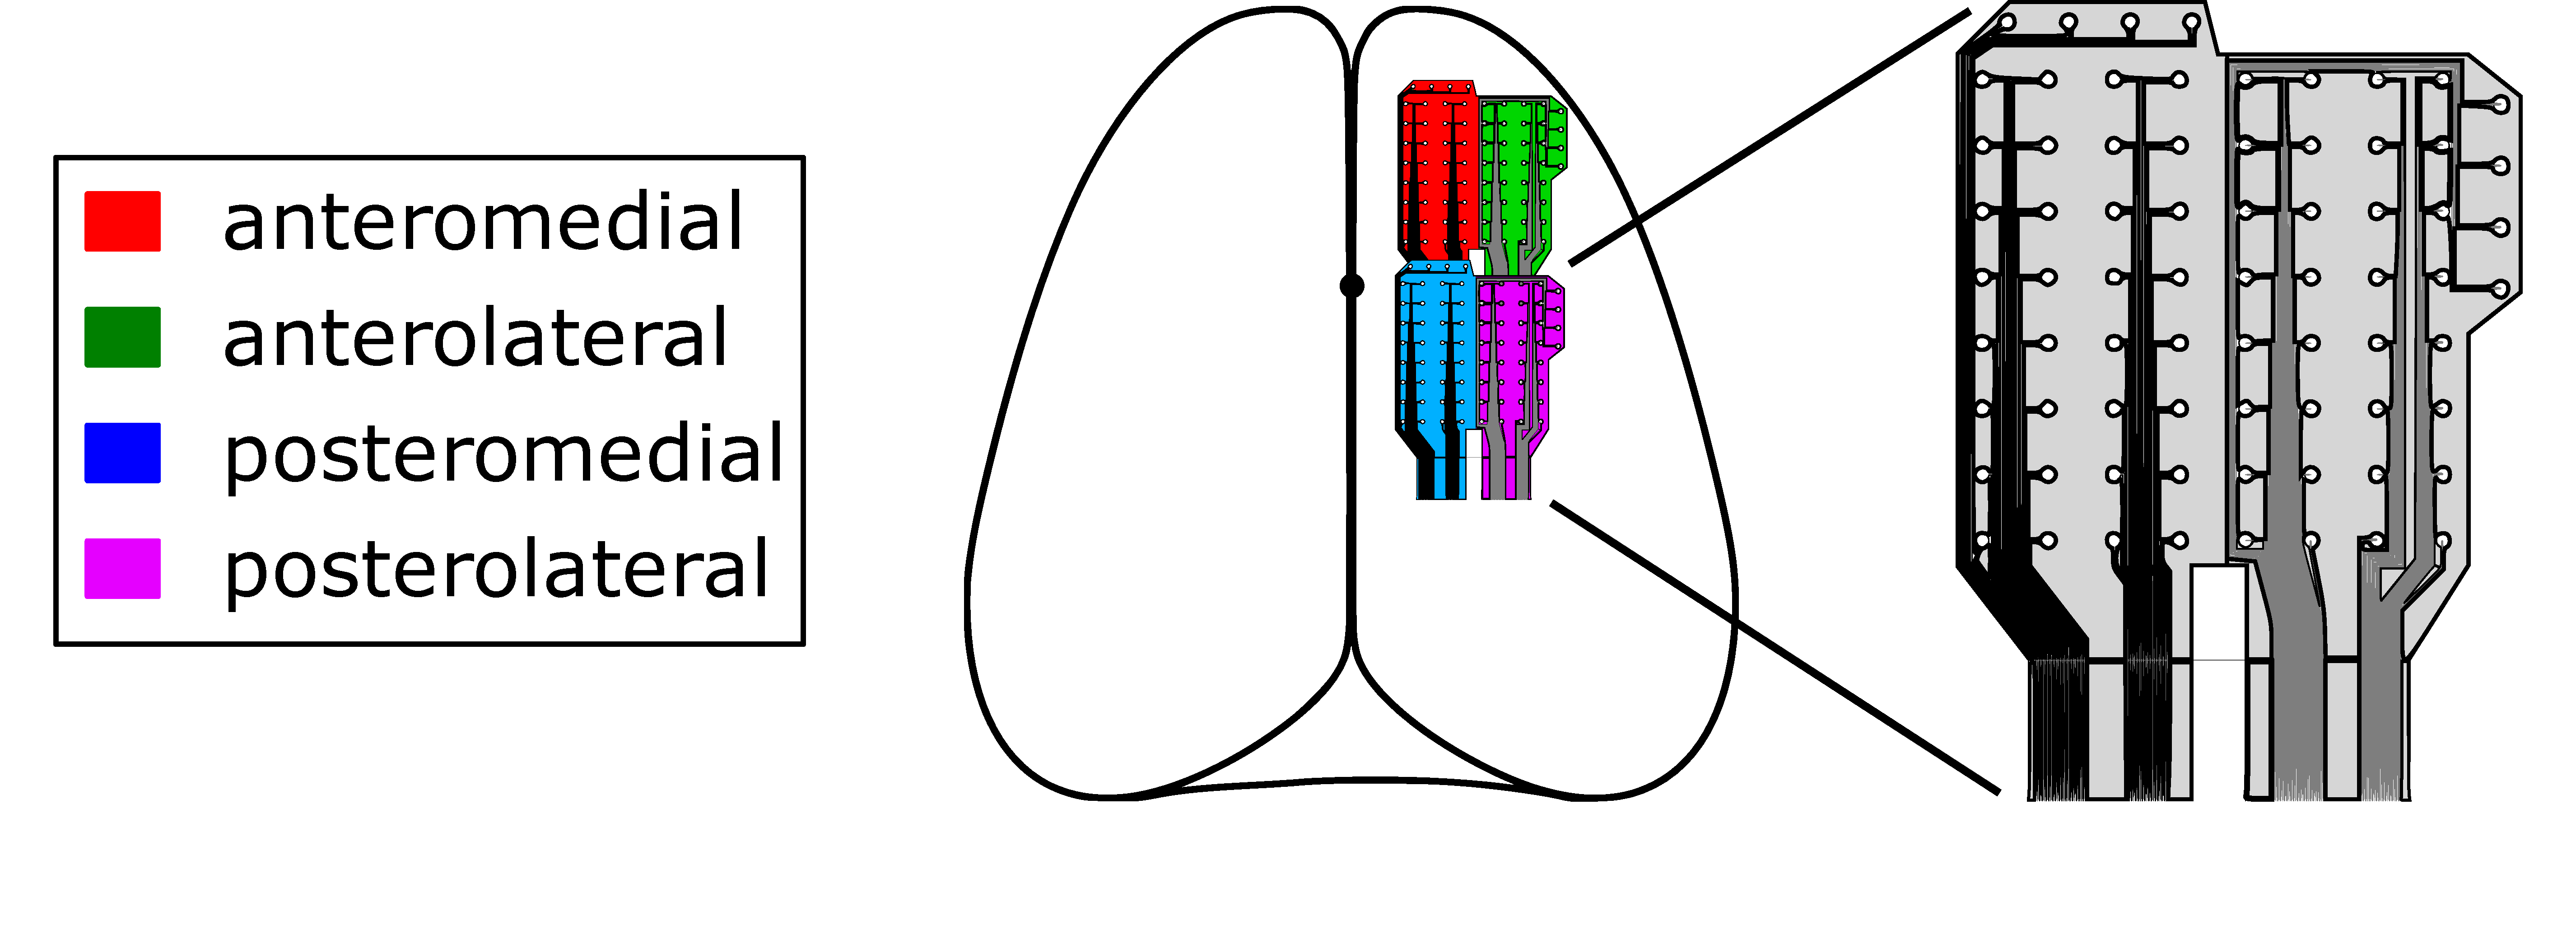
\includegraphics[width=0.5\textwidth]{elements/ecog_simplified_cortex}};
  \node[draw=none,above left=-5.5mm and -1.5mm of ecog_simplified_cortex] {A};

  \node[draw=none,below=-4mm of ecog_simplified_cortex] (ecog_step_erp_jpak74) {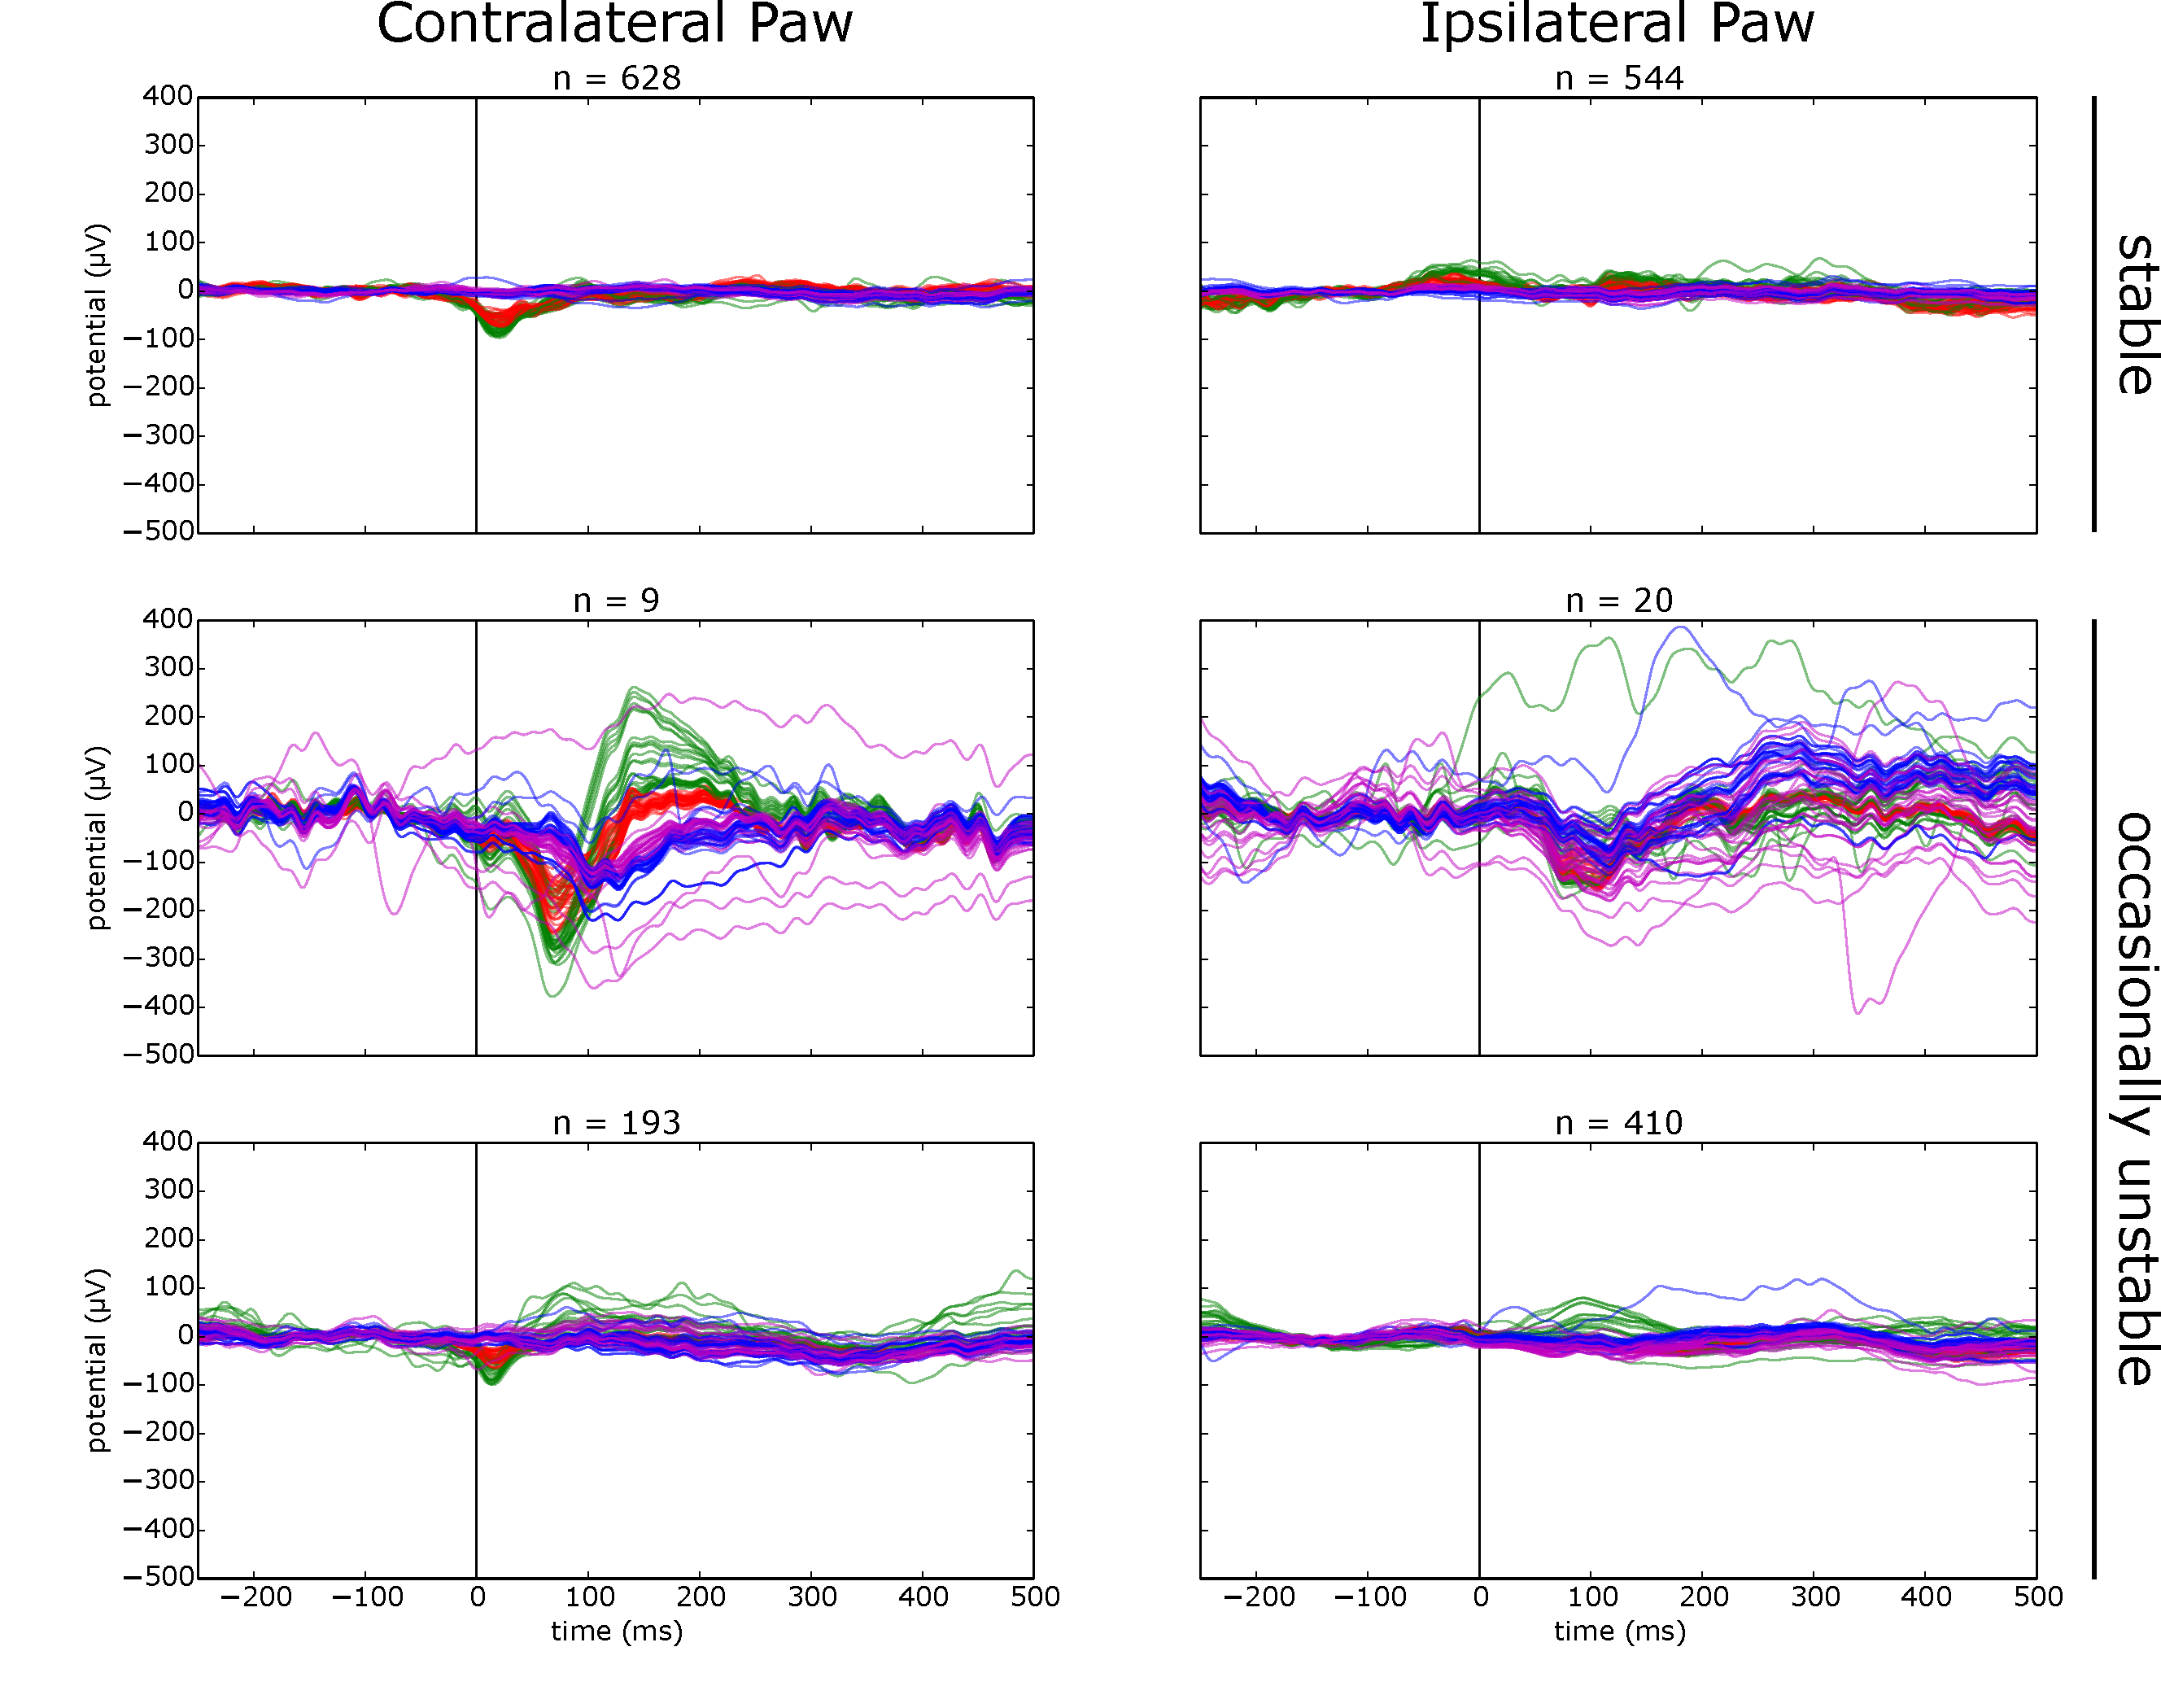
\includegraphics[width=\textwidth]{elements/ecog_step_erp_jpak74}};
  \node[draw=none,above left=-5.0mm and -11mm of ecog_step_erp_jpak74] {B};
  
  \node[draw=none,below left=-7mm and -11.95cm of ecog_step_erp_jpak74] (ecog_step_erp_jpak74_frames) {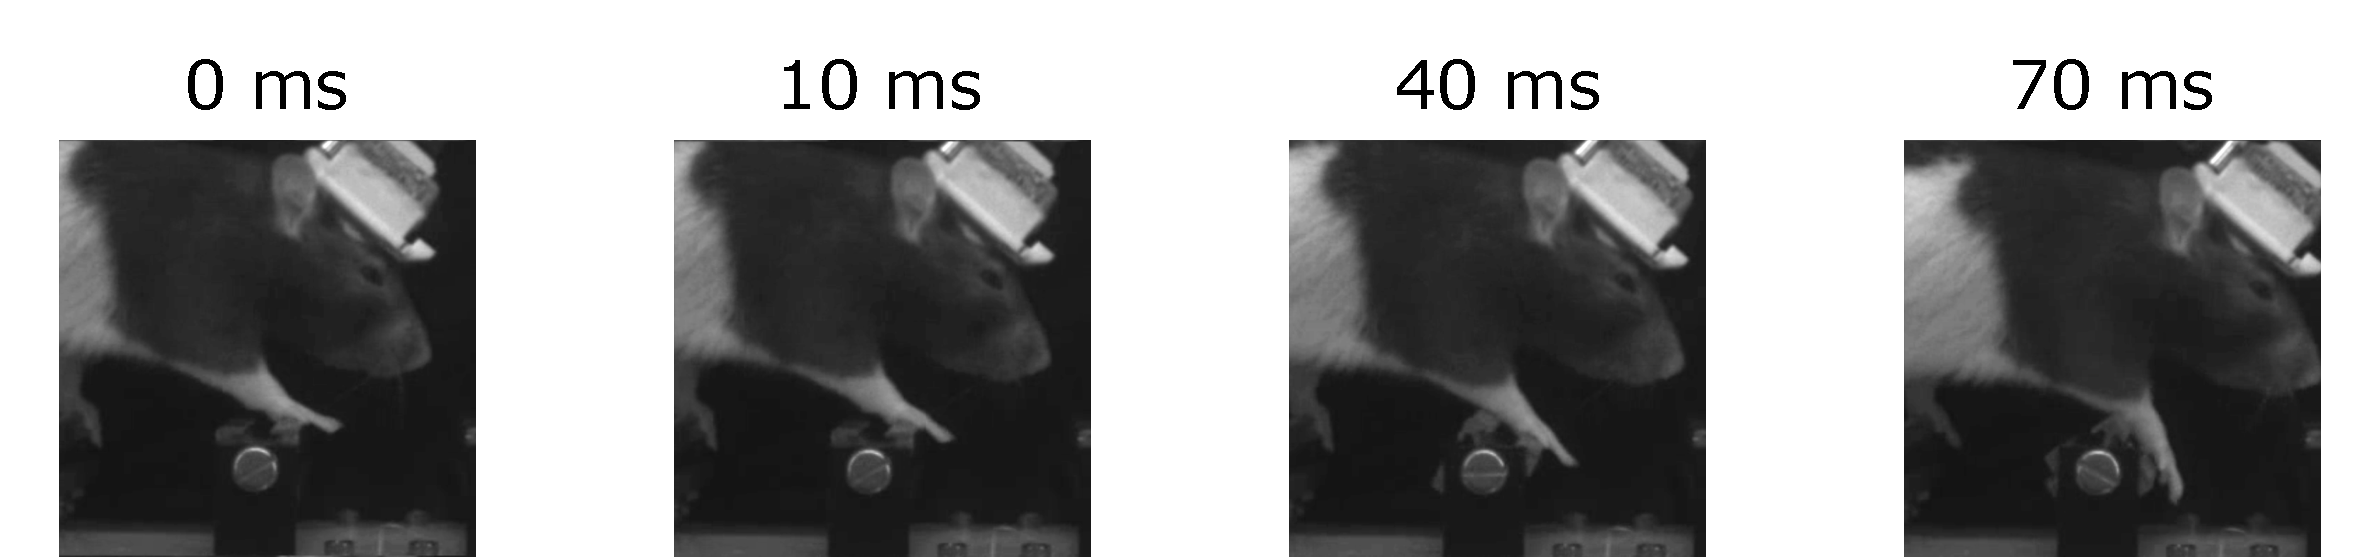
\includegraphics[width=0.9\textwidth]{elements/ecog_step_erp_jpak74_frames}};
  \node[draw=none,above left=-7mm and -2mm of ecog_step_erp_jpak74_frames] {C};
\end{tikzpicture}
\end{document}